\documentclass[a4paper,12pt]{article}
\usepackage[utf8]{inputenc}
\usepackage{xcolor}
\usepackage[english]{babel}  
\usepackage{amsmath,amsfonts,amssymb,amsthm,mathtools} 
\usepackage{wasysym}
\usepackage[pdftex]{graphicx}
\graphicspath{{images/}}
\DeclareGraphicsExtensions{.pdf,.png,.jpg}
\author{Fedor Chuprakov\\ Moscow Institute of Physics and Technology}
\title{Behaviour of a pitiable rocket flying near to the Earth}
\date{\today}


\begin{document}
\maketitle
\newpage
\subsection*{Abstract}
Nowadays many people know that if one jumps thoughtlesly high, he can get a 
bump. But they all have never thought that tiny rockets feel the same! Imagine 
that you're a tiny ricket and you want to change your direction using our 
planet. Everything goes well until you meet our skrewdy atmosphere: 
it slows you down and you fall and explode! That's a pity. In 
this study we will discuss what tiny rockets can do in such situations.
\subsection*{Introduction}
The process of turning around our rocket is explored in this research.
The theoretical model includes \textbf{Newton's law of universal gravitation
} and \textbf{Barometric formula}. This is enough because other things are left
as self-evident. This was implemented in \textbf{Python} program which 
calculates what would happen under initial conditions like coordinate, 
velocity and impact parameter.
\subsection*{Theoretical model}
As it was already mentioned, was used \textbf{Newton's law of universal gravitation}:

\begin{equation}\label{Newton}
	\textbf{F}=G\cdot \frac{m_1\cdot m_2}{r^3} \cdot \textbf{r}
\end{equation}
Where \textit{$F$} is Newton force, \textit{$m_1$} is the rocket mass,
\textit{$m_2$} is the Earth mass and \textit{$r$} is a distance 
between the rocket and the Earth.\\
And \textbf{Barometric formula} (used when the rocket is in the atmosphere):
\begin{equation}\label{Barometric}
	\rho = \rho_0 \cdot exp \left[ \frac{-g \cdot m \cdot H}{k \cdot T} \right]
\end{equation}
Where \textit{$\rho$} is the density of atmosphere, \textit{$\rho_0$} is the 
density near the surface, \textit{$g$} is the gravitational acceleration, 
\textit{$m$} is mass of an air molecule, \textit{$H$} is the height above
the Earth, k is Boltzmann constant and \textit{$T$} is temperature.\\
Also the \textbf{friction force} acts upon the rocket 
(when the rocket is in the atmpsphere):
\begin{equation}\label{Resistance}
	\textbf{F} = -\frac{1}{2} \cdot c \cdot S \cdot v^2 \cdot \frac{\textbf{v}}{v}
\end{equation}
Where \textit{$F$} is the friction force, \textit{$c$} is the drag coefficient,
\textit{$S$} is the effective square and 
\textit{$v$} is the velocity of the rocket.

\subsection*{Methods}
To model such situation \textbf{Python} code was written. You should use
\colorbox{gray!30}{main.py}. There are two functions to use:
\colorbox{gray!30}{sign\_graph.show()} and 
\colorbox{gray!30}{sign\_graph.test()}. They take two arguments.
The first one \colorbox{gray!30}{impact\_parameter} is a required positional
argument representing the impact parameter (it is measured in the 
Earth radius), another one which represents the absolute value of the
initial velocity is a optional keyword argument with the default value 15 pixel 
per second and is referred to as \colorbox{gray!30}{speed}. 
Function \colorbox{gray!30}{sign\_graph.show()} shows how it happens, 
function \colorbox{gray!30}{sign\_graph.test()} finds the optimal 
\textit{impact parameter} in \textit{$O_{0.1}(impact\_parameter)$}.
\subsection*{Results}
Here are the findings of the study. The optimal value if $\textit{speed} = 0.1$ of the \textit{impact parameter} 
is $1.3962 \cdot R_{Earth}$ if the influence of the atmosphere is taken into account 
and $1.3947 \cdot R_{Earth}$ otherwise.
\subsection*{Conclusion}
As it can be seen, the influence of the atmosphere is not that significant 
($\approx 0.1\%$). Nevertheless, since that moment all tiny rockets can 
use this project to fly happily and not be confused.
\subsection*{References}
Author's own physics knowledge and very strange picture on the next pagen take from \\
http://meteoinfo.ru/about/glossary/4806-2012-03-11-20-40-41
\newpage
\begin{figure}[h]
	\center{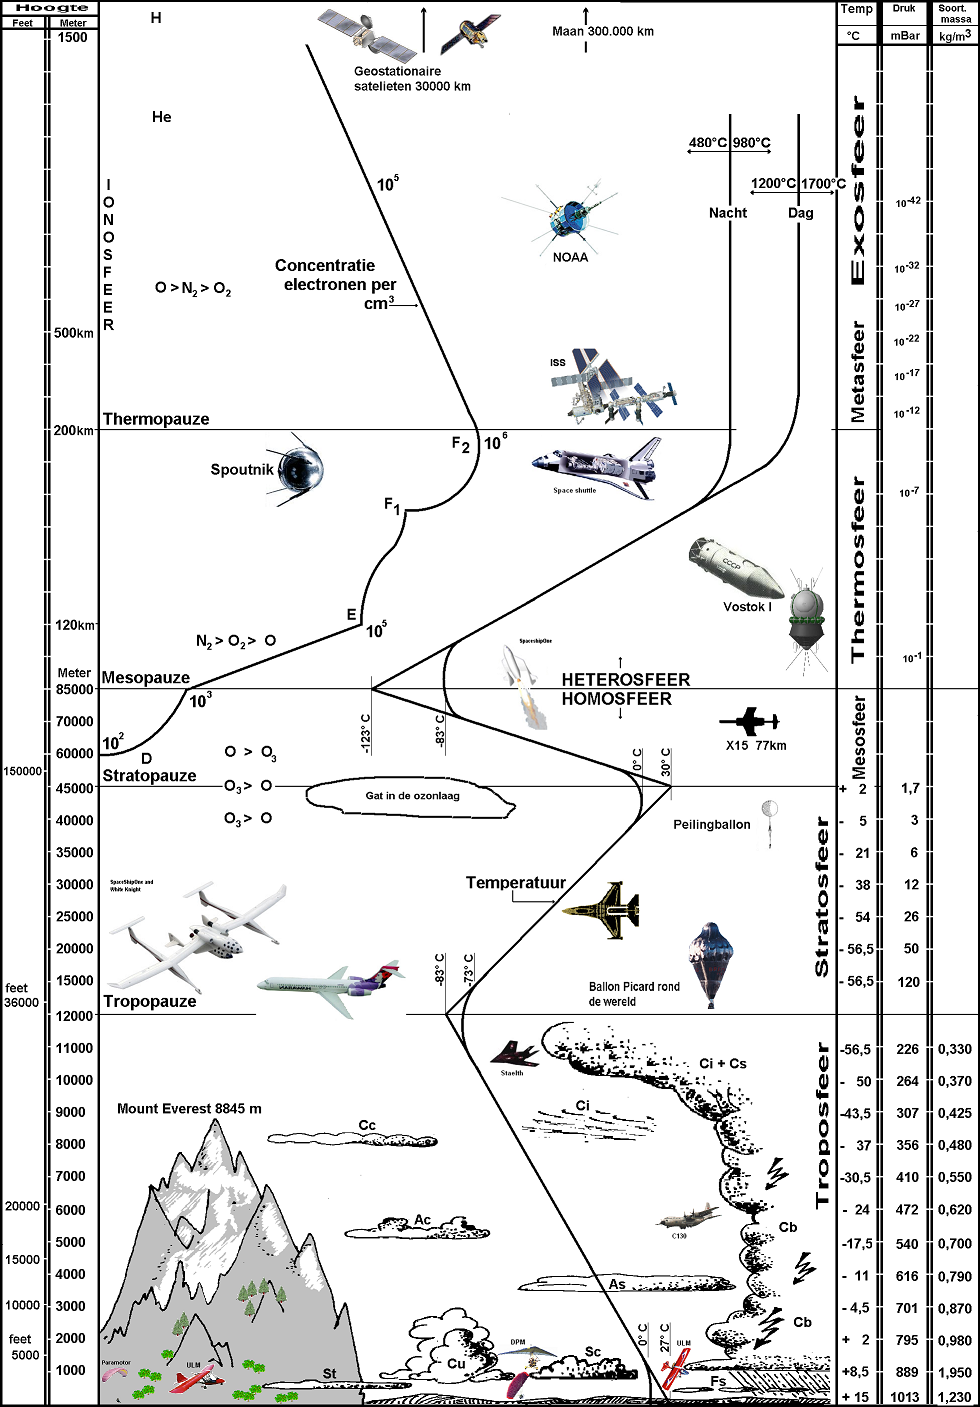
\includegraphics[width=1\linewidth]{atm}}
	\caption{Yeah man you're not mistaken this is the right picture you need to look at so how do you feel mmm? Quite an unexpected function isn't it?}
	\label{ris:athmosphere_vert_struct}
\end{figure}
\end{document}
